\chapter{Design}\label{Design}

<this disseration aims to serve as a guide for security researchers and service operator on the viablity of distributed ech>
<during the course of this project, a system design was formulated and iteratively refined>
<the main parts of the design considered are its deployment schema and protecting traffic>

<in this chapter, we will study the determined solution as well as the challenges that motivated its design>
<this consists of a overview of purposed system followed by an examination of its individual components>



\section{Problem Overview}

<ech split mode serves as a bases for distributed deployment, but makes no attempt to address the implications of servers being operated by separate organisations and located across a public network>
<to do so, we must consider a number of challenges faced by this situation to enable co-operation and secure functioning>
<this paper purposes a loose network of tls servers all acting as ech providers for each other which proxy connections to the true origin server, as depicted in Fig.~\ref{distributed_ech_figure}>

\begin{figure}[ht]
\centerline{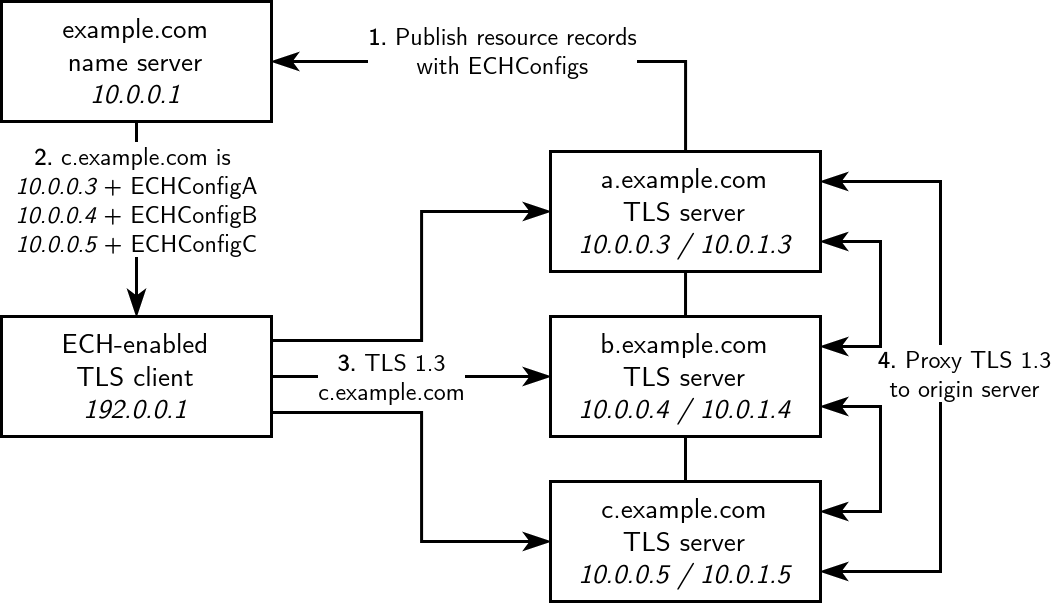
\includegraphics[width=160mm]{images/distributed-ech.png}}
\caption[Example distributed ECH deployment]{<>}
\label{distributed_ech_figure}
\end{figure}

<parallel to the operation of ech split mode>
<loose network must publish appropriate resource records such that clients choose to query any of them for any of their domains>
<all providers listens on their public facing network interface for with ClientHelloOuter>
<providers also listens on a virtual private network interface they are all a part of for actual connections>
<clients resolve requested domain using DoH and then use round robin or other selection process to uniformly choose one of the providers at random with the correct echconfig>
<client begins establishment to the requested via the selected provider using the providers echconfig>
<as in ech split mode, the provider decrypts the ClientHelloInner to retrieve the actual domain requested>
<the provider maps the domain to the true origin server and proxies the clients connection over a backend communication network to the origin server>
<the origin server listening on the vpn interface completes the tls handshake with the client through the provider>
<this connection is end-to-end encrypted, so the provider does not mitm>

<the design challenges can be split into two topics, mechanism for distribution and traffic obfuscation>
<the distribution mechanism deals with a couple designs for the a dns publication schema so compatible clients follow the above process, and the networking required for tls servers to communicate with each other>
<this considers load distribution, echconfig and stream proxying over a virtual private network>







\section{Distribution Mechanism}

<distribution is based on two parts>
<first, clients need to be able to select from several options provided by a dns query>
<second, co-oerating tcp servers need to be able to forward connections to each other based on the decrypted ClientHelloInner>

\subsection{DNS Publication Schema}

<one approach: shared echconfig with round robin A resource records>
<load is evenly distributed across servers because client uses round robin on selected A rrs>
<but requires shared secrets between all servers as there is no way to specify which ech key is associated with which host>
<another approach: using alternative endpoints to associate ech keys with individual servers>
<load is evenly distributed across servers due to matching priority>
<unfortunately more fine-grained load distribution is not possible without srv resource records adoption>
<we can replicate this using a dynamic dns service, where records are regularly substituted such that load is distributed across servers in a fair manner>

\subsection{TLS Server Co-operation}

<tls servers are physically separate from each other and must communicate over the same network as the client when forwarding the client connection>
<to do this, a virtual private network is established between participating servers>
<servers still listen for normal tls connections on 443 port of the public interface as well as ech-enabled connection>
<ech split mode connections have their ClientHelloInner decrypted and private domain mapped to the actual origin>
<clients connection is forwarded over a virtual private network to the origin server>
<the origin server listening on the vpn interface completes the tls handshake with the client through the provider>







\section{Traffic Obfuscation}

<ech is susceptible>\cite{trevisan2023attacking}
<correlation attacks in low-latency systems like web browsing and video streaming compared to high-latency like email>\cite{levine2004timing}
<rx/tx timing> <packet lengths> <traffic patterns> \cite{defabbia2011analyzing}

\begin{figure}[ht]
\centerline{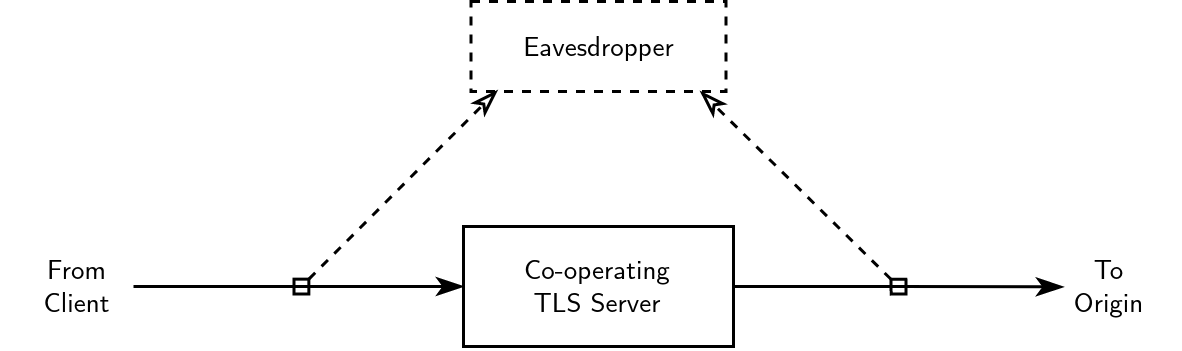
\includegraphics[width=150mm]{images/correlation-attack.png}}
\caption[Diagram of various traffic metrics useful in correlation attacks]{<TODO>}
\label{correlation_figure}
\end{figure}

<traffic obfuscation techniques lead "to disrupt the patterns">

\subsection{Normalisation}

<shannon and perfect secrecy: removal of all identifying features>
<injection of dummy traffic to fill bandwidth gaps>
<impracticality in civilian environments due to required bandwidth>

\subsection{Pacing and Mixing}

<while not perfect, many practical techniques exist to mask traffic with minimal impacts>
<padding packets themselves to prevent packet length correlation>
\cite{yu2012predicted}
<to disrupt timing-based correlation attacks, delays and slotting (aka pacing) can be used>
<to disrupt deep packet inspection, other packet-based correlation attacks (traffic patterns), traffic mixing can be used>
\cite{fu2003analytical, fu2003effectiveness}
<a simple technique is packet duplication, where a similar packet is sent to every peer>

% TODO: likely a comparison table or graph from info theory
% \begin{figure}[ht]
% \centerline{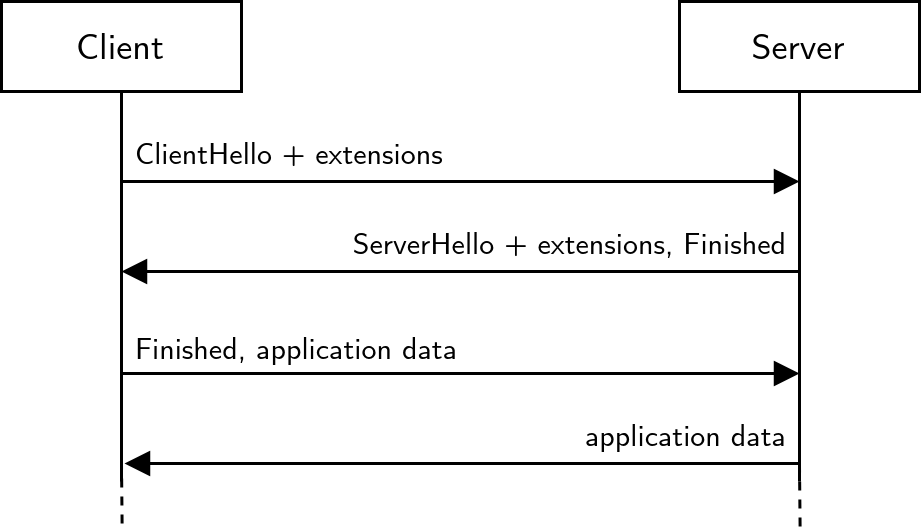
\includegraphics[width=120mm]{images/tls-handshake.png}}
% \caption[TODO technique comparision]{<TODO>}
% \label{noise_figure}
% \end{figure}





\section{Summary}

<it fulfills the desired design criteria>
<we use dns https rrs to distributed load across multiple ech providers>
<separate echconfigs can be used be each server as the ech key is associated with the server>
<an alternative strategy exists that is more robust but requires shared echconfig>
<a virtual private network between co-operating servers is used to allow peer communication>
<ech split mode is vulnerable to correlation attacks>
<but techniques exist to defend against attacks>
